\documentclass[aspectratio=169]{ctexbeamer}
\setbeamertemplate{bibliography item}{\insertbiblabel}
\usetheme{Madrid}
\input{tuna_color.tex}
\usepackage{graphicx}
\usepackage{algpseudocode}
\usepackage{float}
\usepackage{listings}
\usepackage{booktabs}
\usepackage{mathtools}
\usepackage{hyperref}
\usepackage{url}
\usepackage{tikz}
\usetikzlibrary{calc}
\usetikzlibrary{arrows}
\usetikzlibrary{shapes}

\renewcommand{\d}{\mathrm{d}}


\title{Machine Block Placement}
\subtitle{code layout optimizations.}
\author{龙英池}

\input{section_pages.tex}
\input{lst_riscv.tex}
\renewcommand{\lstlistingname}{代码}


% define some basic colors
\definecolor{mauve}{rgb}{0.58,0,0.82}


\setmonofont{Consolas}

\lstset{
% listings sonderzeichen (for german weirdness)
literate={ö}{{\"o}}1
{ä}{{\"a}}1
{ü}{{\"u}}1,
basicstyle=\tiny\ttfamily,                    % very small code
breaklines=true,                              % break long lines
commentstyle=\itshape\color{green!50!black},  % comments are green
keywordstyle=[1]\color{blue!80!black},        % instructions are blue
keywordstyle=[2]\color{orange!80!black},      % sections/other directives are orange
keywordstyle=[3]\color{red!50!black},         % registers are red
stringstyle=\color{mauve},                    % strings are from the telekom
identifierstyle=\color{teal},                 % user declared addresses are teal
frame=l,                                      % black line on the left side of code
language=[RISC-V]Assembler,                   % all code is RISC-V
tabsize=4,                                    % indent tabs with 4 spaces
showstringspaces=false                        % do not replace spaces with weird underlines
}

\lstdefinestyle{mystyle}
{
backgroundcolor=\color{backcolour},
commentstyle=\color{codegreen},
keywordstyle=\color{magenta},
numberstyle=\tiny\color{codegray},
stringstyle=\color{codepurple},
basicstyle=\ttfamily\footnotesize,
breakatwhitespace=false,
breaklines=true,
captionpos=b,
keepspaces=true,
numbers=none,
numbersep=5pt,
showspaces=false,
showstringspaces=false,
showtabs=false,
tabsize=2,
frame=none
}

\lstset{style=mystyle,language=C++}

\begin{document}
\frame{\titlepage}

\begin{frame}
    \frametitle{目录}
    \tableofcontents
\end{frame}

\section{代码布局(Code Layout)}

\begin{frame}[fragile]
    \frametitle{什么是代码布局}
    指令连续地、有顺序地储存在内存中。LLVM中,这些优化过程抽象成控制流图中的基本块(Basic Block, BB)的排列方式。

    \begin{columns}
        \begin{column}{0.2\textwidth}
            \centering
            C Codes:
            \begin{lstlisting}
if (a <= b)
    c = 1;\end{lstlisting}
        \end{column}
        \begin{column}{0.5\textwidth}
            \begin{verbatim}
; a is in rax
; b is in rdx
; c is in rcx
cmp rax, rdx
ja .label
mov rcx, 1
.label:
            \end{verbatim}
        \end{column}
    \end{columns}
\end{frame}

\begin{frame}
    \frametitle{机器代码布局优化}
    基于机器相关的,代码布局的优化主要包含,基本块放置(Basic block placement)、基本块对齐(Basic block alignment)、冷热代码分离(Hot-Cold Splitting)\cite{bakhvalov-2019}.
    \begin{figure}
        \centering
        \includegraphics[width=0.31\textwidth]{images/layout_compare.png}
        \caption{两种不同布局的优劣\cite{cooper2011engineering}}
    \end{figure}

\end{frame}


\begin{frame}[fragile]
    \frametitle{基本块放置}

    \begin{columns}
        \begin{column}{0.3\textwidth}
            \centering
            C Codes:
            \begin{lstlisting}
// hot path
if (cond)
    coldFunc();
// hot path again\end{lstlisting}
        \end{column}
        \begin{column}{0.65\textwidth}
            \begin{figure}
                \centering
                \includegraphics[width=1.\textwidth]{images/hot_cold_placement.jpg}
                \caption{布局优化示例}
            \end{figure}
        \end{column}
    \end{columns}
    \begin{itemize}
        \item 不进行分支跳转往往比跳转代价更低(maintain fall through)
        \item 更好地利用 Cache ($\mu$op-cache) (局部性)
    \end{itemize}

\end{frame}


\section{代码块放置(Block Placement)}

\begin{frame}
    \frametitle{控制流图链剖分}

    首先对CFG建立链剖分,建立的原则是,经常被执行的边被放在一起,形成一条链(Chain)。

    一条链包含一个或多个基本块(BB),并且每个路径都有一个优先级(priority)决定了他们在最终的代码布局中的情况。

    \begin{figure}
        \centering
        \includegraphics[width=0.7\textwidth]{images/hld.png}
        \caption{\cite{unknown-author-2022}轻重链剖分,树上链剖分的一种}
    \end{figure}

\end{frame}


\begin{frame}[fragile]
    \frametitle{Kruskal ? Prim ?}

    CFG没有树这么好的性质,CFG是一个有向图。构建链的方法是每次从边集合中选一条没有被选中的边(按照边的权重顺序),然后形成链状结构。

    \begin{figure}
        \centering
        \includegraphics[width=0.3\textwidth]{images/example_cfg.png}
        \caption{CFG的一个例子\cite{cooper2011engineering}}
    \end{figure}



\end{frame}

\begin{frame}
    \frametitle{CFG上的贪心启发式链剖分 (Greedy heuristic chain div on CFGs)}

    \begin{algorithmic}
        \State $E$ $\gets$ | edges |
        \For{each block b}
        \State make a degenerate chain, $d$, for $b$
        \State priority($d$) $\gets$ $E$
        \EndFor
        \State $P \gets 0$
        \For{each CFG edge $<x, y>, x \neq y$, in decreasing freq order}
        \State $ t \gets $ priority($a$)
        \State append $b$ onto $a$
        \State priority($a$) $\gets$ $\min$ ($t$, priority($b$), $P$++)
        \EndFor
    \end{algorithmic}


\end{frame}

\begin{frame}
    \frametitle{CFG上的贪心启发式链剖分 (Greedy heuristic chain div on CFGs)}

    \begin{columns}
        \begin{column}{0.3\textwidth}
            \begin{figure}
                \centering
                \includegraphics[width=1.0\textwidth]{images/example_cfg.png}
                \caption{CFG的一个例子\cite{cooper2011engineering}}
            \end{figure}
        \end{column}
        \begin{column}{0.6\textwidth}
            \begin{figure}
                \centering
                \includegraphics[width=1.0\textwidth]{images/greedy.png}
                \caption{算法每个过程选择的边,和对应的边集}
            \end{figure}
        \end{column}
    \end{columns}

\end{frame}


\begin{frame}
    \frametitle{基于WorkList组合最终的代码布局(Code Layout)}

    \begin{algorithmic}
        \State $t$ $\gets$ chain headed by the CFG entry node
\State $WorkList$ $\gets$ $\lbrace(t, priority(t))\rbrace$ $ \qquad \Leftarrow$ Heap\cite{forsythe1964algorithms}
        \While{$WorkList \neq \emptyset$}
        \State remove a chian $c$ of lowest priority from $WorkList$
        \For{each block $x$ in $c$ in chain}
        \State place $x$ and the end of assembly codes
        \EndFor
        \For{each block $x$ in $c$}
        \For{each edge $<x, y$ where $y$ is unplaced}
        \State $t \gets $ chain containing $<x, y>$
        \If{$(t, priority(t)) \notin WorkList$}
        $WorkList \gets WorkList \bigcup \lbrace (t, priority(t)) \rbrace$
        \EndIf
        \EndFor
        \EndFor
        \EndWhile
    \end{algorithmic}

\end{frame}


\begin{frame}
    \frametitle{Example}
    \begin{columns}
        \begin{column}{0.5\textwidth}
            \begin{figure}
                \centering
                \includegraphics[width=1.0\textwidth]{images/greedy.png}
                \caption{上一个过程形成的链}
            \end{figure}
        \end{column}
        \begin{column}{0.5\textwidth}
            \begin{figure}
                \centering
                \includegraphics[width=1.0\textwidth]{images/worklist.png}
                \caption{生成最终的代码布局}
            \end{figure}
        \end{column}
    \end{columns}
\end{frame}
\section{LLVM 中如何实现这个算法}


\begin{frame}
    \frametitle{TL; DR}

    算法主体主要实现在 lib/CodeGen/MachineBlockPlacement.cpp

    \vspace{1.5em}

    其中分支概率等信息来源于 Block\{Frequency, ProbabilityInfo\}

    \vspace{1.5em}

    各个 Target 需要实现 \{ analyze, insert, remove \}Branch等虚函数,RISC-V在 5 年前,D40808\cite{llvmriscvimplbranchanalysis2017}实现;两年前,D84833包含了一个间接分支实现 \cite{llvmriscvimplindirect2020}
    \begin{table}
        \begin{tabular}{ccc}
            \toprule
            功能   & 实现                    & 源代码位置                                                                              \\
            \midrule
            边权   & BlockFrequency        & \cite{llvmblockfreqinfoimpl2022}                                                   \\
            块放置  & MachineBlockPlacement & buildCFGChains()\cite{llvmmachineblockplacement2022}                               \\
            块对齐  & MachineBlockPlacement & alignBlocks()\cite{llvmmachineblockplacement2022}                                  \\
            分支分析 & RISCVInstrInfo        & analyzeBranch()\cite{llvmriscvinstrinfo2022}\cite{llvmriscvimplbranchanalysis2017} \\
            \bottomrule
        \end{tabular}
        \caption{各个功能的实现情况和所在的位置}
    \end{table}

\end{frame}

\begin{frame}
    \frametitle{最开始的布局优化Pass - CodePlacementOptPass}

    2009 年10月,此时 LLVM 大仓库还只有 clang、compiler-rt、llvm。这时 LLVM 的布局优化 Pass 还没有基于 Macine-IR,CodePlacementOptPass \cite{llvmcodeplacementopt2009}将一些循环尾部的,无条件跳转到循环首部(back-edges)的块,移动到循环的开头。

    \begin{figure}
        \centering
        \includegraphics[width=0.25\textwidth]{images/slightly_more_involved.png}
        \caption{block\_a可以被提到循环的开头}
    \end{figure}

\end{frame}


\begin{frame}
    \frametitle{LLVM 对 Pettis-Hansen 算法的改进}

    2021年12月,MachineBlockPlacement 的基本功能有了新的改进。D113424\cite{llvmexttspbbl2021} 引入一个方案,来优化已经完成链剖分之后的,生成最终的代码布局的过程。

    \begin{figure}
        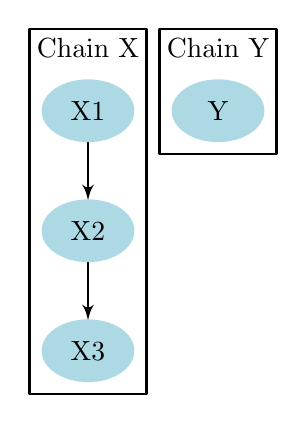
\begin{tikzpicture}[>=latex',line join=bevel,scale=0.6]
    \pgfsetlinewidth{1bp}
    %%
    \begin{scope}
        \pgfsetstrokecolor{black}
        \definecolor{strokecol}{rgb}{0.0,0.0,0.0};
        \pgfsetstrokecolor{strokecol}
        \draw (8.0bp,8.0bp) -- (8.0bp,227.0bp) -- (78.0bp,227.0bp) -- (78.0bp,8.0bp) -- cycle;
        \draw (43.0bp,215.5bp) node {Chain X};
    \end{scope}
    \begin{scope}
        \pgfsetstrokecolor{black}
        \definecolor{strokecol}{rgb}{0.0,0.0,0.0};
        \pgfsetstrokecolor{strokecol}
        \draw (86.0bp,152.0bp) -- (86.0bp,227.0bp) -- (156.0bp,227.0bp) -- (156.0bp,152.0bp) -- cycle;
        \draw (121.0bp,215.5bp) node {Chain Y};
    \end{scope}
    \pgfsetcolor{black}
    % Edge: X1 -> X2
    \draw [->] (43.0bp,159.7bp) .. controls (43.0bp,151.98bp) and (43.0bp,142.71bp)  .. (43.0bp,124.1bp);
    % Edge: X2 -> X3
    \draw [->] (43.0bp,87.697bp) .. controls (43.0bp,79.983bp) and (43.0bp,70.712bp)  .. (43.0bp,52.104bp);
    % Node: X1
    \begin{scope}
        \definecolor{strokecol}{rgb}{0.68,0.85,0.9};
        \pgfsetstrokecolor{strokecol}
        \definecolor{fillcol}{rgb}{0.68,0.85,0.9};
        \pgfsetfillcolor{fillcol}
        \filldraw [opacity=1] (43.0bp,178.0bp) ellipse (27.0bp and 18.0bp);
        \definecolor{strokecol}{rgb}{0.0,0.0,0.0};
        \pgfsetstrokecolor{strokecol}
        \draw (43.0bp,178.0bp) node {X1};
    \end{scope}
    % Node: X2
    \begin{scope}
        \definecolor{strokecol}{rgb}{0.68,0.85,0.9};
        \pgfsetstrokecolor{strokecol}
        \definecolor{fillcol}{rgb}{0.68,0.85,0.9};
        \pgfsetfillcolor{fillcol}
        \filldraw [opacity=1] (43.0bp,106.0bp) ellipse (27.0bp and 18.0bp);
        \definecolor{strokecol}{rgb}{0.0,0.0,0.0};
        \pgfsetstrokecolor{strokecol}
        \draw (43.0bp,106.0bp) node {X2};
    \end{scope}
    % Node: X3
    \begin{scope}
        \definecolor{strokecol}{rgb}{0.68,0.85,0.9};
        \pgfsetstrokecolor{strokecol}
        \definecolor{fillcol}{rgb}{0.68,0.85,0.9};
        \pgfsetfillcolor{fillcol}
        \filldraw [opacity=1] (43.0bp,34.0bp) ellipse (27.0bp and 18.0bp);
        \definecolor{strokecol}{rgb}{0.0,0.0,0.0};
        \pgfsetstrokecolor{strokecol}
        \draw (43.0bp,34.0bp) node {X3};
    \end{scope}
    % Node: Y
    \begin{scope}
        \definecolor{strokecol}{rgb}{0.68,0.85,0.9};
        \pgfsetstrokecolor{strokecol}
        \definecolor{fillcol}{rgb}{0.68,0.85,0.9};
        \pgfsetfillcolor{fillcol}
        \filldraw [opacity=1] (121.0bp,178.0bp) ellipse (27.0bp and 18.0bp);
        \definecolor{strokecol}{rgb}{0.0,0.0,0.0};
        \pgfsetstrokecolor{strokecol}
        \draw (121.0bp,178.0bp) node {Y};
    \end{scope}
    %
\end{tikzpicture}
        \caption{需要合并的两个Chain示意}
    \end{figure}

\end{frame}

\begin{frame}
    \frametitle{BOLT - Binary optimization and layout tool}

    Facebook 在 2018 年开源了他们的二进制优化工具 -- BOLT\cite{facebook2018bolt}\cite{panchenko2019bolt}。这个仓库现在已经合并到 LLVM,可以在对编译后的二进制进行基本的重排,冷热代码分离等工作。

    \begin{figure}
        \centering
        \includegraphics[width=0.6\textwidth]{images/perf_improv_clang.png}
        \caption{优化后的Clang}
    \end{figure}

\end{frame}
\section{References}


\begin{frame}[allowframebreaks]
    \frametitle{References}
    \bibliographystyle{ieeetr}
    \bibliography{main.bib}
\end{frame}
\end{document}